\section[Symmetry and Goldstone's theorem${}^*$]{Symmetry and Goldstone's theorem}
\label{section:symmetry}

This section is based on~\autocite{leeSmoothManifolds2012,peskinIntroductionQuantumField1995,weinbergQuantumTheoryFields1995,weinbergQuantumTheoryFields1996}.

Symmetry plays a prominent role in modern physics.
If we can transform a physical state in such a way that the governing equations of this system are unchanged, we call that transformation a \emph{symmetry transformation}.
All such transformations are known as the symmetries of that theory.
The symmetries of a theory encode a lot of physics, such as the presence of conserved quantities and the system's low energy behavior.
We distinguish between internal and external symmetries.
An external symmetry is an active coordinate transformation, such as rotations or translations.
They relate degrees of freedom at different space-time points, while internal symmetries transform degrees of freedom at each space-time point independently.
A further distinction is between global and local symmetry transformations.
Global transformations have one rule for transforming degrees of freedom at each point, which is applied everywhere, while local transformations are functions of space-time.

In classical field theory, symmetries are encoded in the behavior of the Lagrangian when the fields are transformed.
We will consider continuous transformations, which can in general be written as
\begin{equation}
    \varphi(x) \longrightarrow \varphi'(x) = f_t[\varphi](x), \quad t \in [0, 1].
\end{equation}
%
Here, $f_t[\varphi]$ is a functional in $\varphi$, and a smooth function of $t$, with the constraint that $f_0[\varphi] = \varphi$.
This allows us to look at ``infinitesimal'' transformations,
\begin{equation}
    \label{infinitesimal transformation}
    \varphi'(x) = f_\epsilon[\varphi] 
    = \varphi(x) + \epsilon \odv{ f_t[\varphi] }{t}\bigg |_{t=0} + \Oh{\epsilon}.
\end{equation}
%
When considering infinitesimal transformations, we will not always write $ + \Oh{\epsilon}$, but rather consider it implicit.
We will consider internal, global transformations which act linearly on $\varphi$.
For $N$ fields, $\varphi_i$, this can be written
\begin{equation}
    \label{linear field transformation}
    \varphi_i'(x) = \varphi_i(x) + \epsilon \, i V_{ij} \varphi_j(x).
\end{equation}
%
$V_{ij}$ is called the generator of the transformation.
A symmetry transformation of the system is then a transformation in which the Lagrangian left is unchanged, or at most differ by a 4-divergence term.
That is, a transformation $\varphi \rightarrow \varphi'$ is a symmetry if 
\begin{equation}
    \Ell[\varphi'] = \Ell[\varphi] + \partial_\mu K^\mu[\varphi],
\end{equation}
%
where $K^\mu[\varphi]$ is a functional of $\varphi$.\footnote{Terms of the form $\partial_\mu K^\mu$ does not affect the physics, as variational principle $\delta S = 0$ do not vary the fields at infinity. Together with the divergence theorem, this means that such terms do not influence the equations of motion.}
This is a requirement for symmetry in quantum field theory too.
However, as physical quantities in quantum field theory are given not just by the action of a single state but the path integral, the integration measure $\D \varphi$ has to be invariant as well.
If a classical symmetry fails due to the non-invariance of the integration measure, it is called an \emph{anomaly}.

To investigate the symmetry properties of a quantum theory, we explore what constraints a symmetry imposes on the effective action.
To that end, assume 
\begin{equation}
    \D \varphi'(x) = \D \varphi(x), \quad
    S[\varphi'] = S[\varphi].
\end{equation}
%
In the generating functional, such a transformation corresponds to a change of integration variable.
Using the infinitesimal version of the transformation, we may write
\begin{align}
    \nonumber
    Z[J]
    = \int \D \varphi \, \exp{i S[\varphi] + i \int \dd^4 x \,J_i(x) \varphi_i(x)} 
    = \int \D \varphi' \, \exp{i S[\varphi'] + i \int \dd^4 x \, J_i(x) \varphi'_i(x)}
    \\
    = Z[J] + i \epsilon \int \dd^4 x \, J_i(x) \int \D \varphi \, [V_{ij} \varphi_j(x)]  e^{i S[\varphi]},
\end{align}
%
Using \autoref{effective equation of motion}, we can write this as
\begin{equation}
    \label{effective action symmetry requirement}
    \int \dd^4 x \, \fdv{\Gamma[\varphi_J]}{\varphi_i(x)} \, V_{ij}\ex{\varphi_j(x)}_J = 0.
\end{equation}
%
This constraint will allow us to deduce the properties of a theory close to the ground state, only using information about the symmetries of the theory.


The archetypical example of an internal, global, and continuous symmetry is the linear sigma model, which we will use as an example throughout this section.
The linear sigma model is made up of $N$ real scalar fields $\varphi_i$, whose Lagrangian is
\begin{equation}
    \Ell[\varphi] 
    = \frac{1}{2} \partial_\mu \varphi_i(x) \partial^\mu \varphi_i(x) - \Ve(\varphi),
    \quad \Ve(\varphi) = - \frac{1}{2} \mu^2 \varphi_i(x)\varphi_i(x)
    + \frac{1}{4} \lambda [\varphi_i(x) \varphi_i(x)]^2.
\end{equation}
%
This system is invariant under the rotation of the $N$ fields into each other,
\begin{equation}
    \varphi_i \longrightarrow \varphi_i' = M_{ij} \varphi_j,
    \quad M^{-1} = M^{T}.
\end{equation}
%
The set of all such transformations forms the Lie group $\text{O}(N)$.
Lie groups will be discussed in the next section.
For $N = 2$, and $\mu^2, \lambda > 0$ we get the ubiquitous Mexican hat potential, as illustrated in \autoref{fig:Mexican hat}.

\begin{figure}[ht]
    \centering
    \includegraphics[width=0.6\textwidth]{figurer/mexican_hat.pdf}
    \caption{The Mexican hat potential is the classical potential $\Ve$ for the $N=2 $ linear sigma model.}
    \label{fig:Mexican hat}
\end{figure}


% Lie groups

\subsection{Nöther's theorem}

One of the most profound consequences of symmetry in physics is the appearance of conserved quantities.
Assume we have a set of fields $\varphi_i$. Nöther's theorem tells us that if the Lagrangian $\Ell[\varphi_i]$ has a continuous symmetry, then there is a corresponding conserved current~\autocite{carrollSpacetimeGeometryIntroduction2019,peskinIntroductionQuantumField1995}.
Consider an infinitesimal transformation,
\begin{equation}
    \varphi_i(x) \longrightarrow \varphi_i'(x)
    = \varphi_i(x) + \delta \varphi_i(x),.
\end{equation}
%
Applying this transformation to the Lagrangian will in general change its form,
\begin{equation}
    \Ell[\varphi] \rightarrow \Ell[\varphi']
    = \Ell[\varphi] + \delta \Ell.
\end{equation}
%
We assume this transformation is a symmetry, i.e.,
\begin{equation*}
    \delta \Ell = \partial_\mu K^\mu.
\end{equation*}
%
By considering the Lagrangian as a function of the field and its derivatives, $\Ell = \Ell(\varphi_i, \partial_\mu \varphi_i)$, we can write the difference term as a Taylor expansion around $(\varphi_i, \partial_\mu \varphi_i)$,
\begin{align}
    \delta \Ell
    = \pdv{\Ell}{\varphi_i} \delta \varphi_i
    + \pdv{\Ell}{(\partial_\mu \varphi_i)} \delta (\partial_\mu \varphi_i),
\end{align}
%
where $\delta (\partial_\mu \varphi_i) = \partial_\mu \varphi_i' - \partial_\mu \varphi_i$.
By the linearlity of the derivative,
\begin{equation}
    \delta (\partial_\mu \varphi_i)
    = \partial_\mu \varphi_i' - \partial_\mu \varphi_i
    = \partial_\mu (\varphi_i' - \varphi_i)
    = \partial_\mu \delta \varphi_i.
\end{equation}
%
With this, and the Euler-Lagrange equations
\begin{equation}
    \partial_\mu \pdv{\Ell}{(\partial_\mu \varphi)} - \pdv{\Ell}{\varphi_i} = 0,
\end{equation}
%
we can rewrite
\begin{equation}
    \delta \Ell = \left( \partial_\mu \pdv{\Ell}{(\partial_\mu \varphi_i)} \right) \delta \varphi_i
    + \pdv{\Ell}{(\partial_\mu \varphi_i)} (\partial_\mu \delta \varphi_i)
    = \partial_\mu \left(\pdv{\Ell}{(\partial_\mu \varphi_i)} \delta \varphi_i\right)
\end{equation}
%
If we define the current
\begin{equation}
    j^\mu = \pdv{\Ell}{(\partial_\mu \varphi_i)} \delta \varphi_i(x) - K^\mu,
\end{equation}
%
then 
\begin{equation}
    \partial_\mu j^\mu = \delta \Ell - \delta \Ell = 0.
\end{equation}
%
This is Nöther's theorem; a continuous symmetry implies the existence of a conserved current.

The current flux through some spacelike surface $V$ defines a conserved charge. The surface of constant time in some reference frame has the normal vector $n_\mu = (1, 0, 0, 0)$, so the charge is
\begin{equation}
    Q = \int_V \dd^4 x \, n_\mu j^\nu = \int_V \dd^3 x \, j^0.
\end{equation}
%
We can then use the divergence theorem.
Assume $\partial V$ is the boundary of $V$, which has the space-like normal vector $k_i$, and that the current falls of quickly towards infinity.
Then
\begin{equation}
    \pdv{t} Q = - \int_V \dd^3 x \, \partial_i j^i = - \int_{\partial V} \dd^2 x\, k_i j^i = 0,
\end{equation}
%
proving that the charge is conserved.

\subsection{Goldstone's theorem}

A symmetry transformation will leave the governing equation of a theory unchanged.
This, however, does not imply that physical states, such as the ground state, are invariant under this transformation.
The $N = 2$ linear sigma model illustrates this.
If we assume the ground state $\varphi_{0}$ is translationally invariant, then it is given by minimizing the effective potential, of which the classical potential, $\Ve$, is the leading order approximation.
This potential is illustrated in \autoref{fig:Mexican hat}.
The ground state is therefore given by any of the values along the brim of the potential.
If we, without loss of generality, choose $\varphi_0 = (0, v)$ as the ground state, then any rotation will change this state.
We say that the symmetry has been \emph{spontaneously broken}.

To explore this in a general context, assume a theory of $N$ real scalar fields $\varphi_i$ are invariant under the actions of some Lie group, $G$.
A symmetry $g \in G$ is broken if the vacuum expectation value of the original fields and the transformed fields differ.
That is, if
\begin{equation}
    \ex{\varphi}_0 \neq \ex{\varphi'}_0 = \ex{g \varphi}_0
\end{equation}
%
We can now exploit what we learned about Lie groups to write the infinitesimal transformation as
\begin{equation}
    \ex{\varphi'}_0 = \ex{\varphi}_0 + i \epsilon \eta_\alpha T_\alpha \ex{\varphi}_0.
\end{equation}
%
Let $x_i$ be the set of generators corresponding to broken symmetries, i.e.,
\begin{equation}
    x_i \ex{\varphi}_0 \neq 0.
\end{equation}
%
These are called the \emph{broken generators}.
The remaining set of generators $t_a$, which obey
\begin{equation}
    t_a \ex{\varphi}_0 = 0,
\end{equation}
%
are called unbroken, and generate a subgroup $H \subset G$ as the set of symmetry transformations of the vacuum is a group.

In \autoref{effective action symmetry requirement} we found that, if $V$ is the generator of some symmetry, then the effective action obeys
\begin{equation}
    \int \dd^4 x\, \fdv{\Gamma[\varphi_J]}{\varphi_i} V_{ij} \ex{\varphi_j}_0 = 0,
\end{equation}
%
We now differentiate this expression with respect to $\varphi_k(y)$ and evaluate it in the vacuum, which gives
\begin{equation}
    \int \dd^4 x \, \fdv{\Gamma[\varphi_0]}{\varphi_k(y), \varphi_i(x)}
    V_{ij} \ex{\varphi_j}_0 = 0.
\end{equation}
%
With the assumption that the ground state is constant, we get 
\begin{equation}
    \pdv{\Veff}{\varphi_k, \varphi_i} \, V_{i j} \ex{\varphi_j}_0 = 0.
\end{equation}
%
This is trival for unbroken symmetries, as $t^a_{ij}\ex{\varphi_j}_0 = 0$ by definition.
However, in the case of a broken symmetry, the second derivative of the effective potential has an eigenvector $x^\ell_{ij} \ex{\varphi_j}_0$ with a zero eigenvalue for each broken generator.
Here, $\ell$ label the set of generators, while $(ij)$ are the indices corresponding to field-components $\varphi_i$.
In \autoref{Effective action inverse propagator}, we found that the second derivative of the effective action is the inverse propagator,
\begin{equation}
    D^{-1}_{ij}(x,y) 
    = \fdv{\Gamma[\varphi_0]}{\varphi_i(y), \varphi_j(x)}
    = \int \frac{\dd^4 p}{(2 \pi)^4} e^{-ip(x - y)} \, \tilde D^{-1}_{ij}(p).
\end{equation}
%
Using this, we can write
\begin{equation}
    \tilde D^{-1}_{i j}(p=0) \, x^\ell_{jk} \ex{\varphi_k}_0 
    = 0.
\end{equation}
%
Zeros of the inverse propagator correspond to the physical mass of particles.
In Lorentz-invariant systems, each zero-eigenvalue vector corresponds to a masses particle, called a Goldstone boson.\footnote{ The particles are bosons due to the bosonic nature of the transformations, $g$. If the generators are Grassmann numbers, the resulting particles, called goldstinos, are fermions.}
This means there are $n_G = \dim G -\dim H$ zero-mass modes.
In general, the counting of massless modes is complicated and depends on the dispersion relation of the particles at low momenta.
Systems with Goldstone bosons with quadratic dispersion relation, that is $E \propto |\vv p|^2$ when $\vv p \rightarrow 0$, often exhibit a lower number of massless modes.
An example is ferromagnets, where the $\mathrm{SU}(2)$ rotational symmetry is broken down to $\mathrm{U}(1)$ when they align along one axis. 
This corresponds to two broken generators, yet the system exhibits only one massless mode~\autocite{braunerSpontaneousSymmetryBreaking2010}.

\begin{figure}[ht]
    \centering
    \hspace*{2.5cm}
    \includegraphics[width=.6\linewidth]{figurer/mexican_hat_zoom.pdf}
    \caption{Excitations along the brim does not cost any energy, as the potential is flat, unlike excitations in the radial direction.}
    \label{fig:Mexican hat zoom}
\end{figure}

The linear sigma model gives an intuition for the Goldstone mode.
In the case of $N = 2$, the symmetry of the Lagrangian are rotations in the plane.
As the ground state is a point along the ``brim'' of the hat, this rotational symmetry is broken.
However, any excitations in the angular direction do not cost any energy, which is indicative of a massless mode.
This is illustrated in \autoref{fig:Mexican hat zoom}.
In this example, the original symmetry group is one-dimensional, so there are no unbroken symmetries.
Consider instead the $N=3$ linear sigma model, which has the three-dimensional symmetry group $\SO(3)$, rotations of the sphere.
We see that the ground state is left invariant under a subgroup of the original symmetry transformations.
The ground state manifold of this system, the set of all states that minimizes the effective potential, is then a sphere.
When the system chooses one single ground state, this symmetry is broken, but only for two of the generators. 
The generator for rotations around the ground state leaves that point unchanged and is thus an unbroken symmetry.
Any excitations in the direction of the broken symmetries do not cost energy, as it is in the ground state manifold.
On the other hand, the unbroken symmetry does not correspond to an excitation.
This is illustrated in \autoref{fig:ground state manifold}.

\begin{figure}[h]
    \centering
    \includegraphics[width=.35\linewidth]{figurer/SU(3).pdf}
    \caption{Excitations for the $N=3$ sigma model. Two of the symmetries are broken, while rotations around the groundstate leaves the system unchanged.}
    \label{fig:ground state manifold}
\end{figure}
